\documentclass{article}

% Word count progress (only counting the content, not the copy of the interim
% report)
% 2022-04-14, 1200 words, 2.5 pages
% 2022-04-15, 1900 words, 4 pages

\usepackage[margin=0.55in,bottom=0.75in]{geometry}
%\usepackage[margin=0.75in]{geometry}
\usepackage{titlesec}
\usepackage{datetime}
\usepackage{graphicx}
\usepackage{array}
\usepackage{tabularx}
\usepackage{amssymb}
\usepackage{amsmath}
\usepackage{amsfonts}
\usepackage{makecell}
% Format footnotes (bottom of page, reset counter at every page break, use
% symbols instead of numbers)
\usepackage[bottom,perpage,symbol*]{footmisc}
\usepackage{csquotes}
\usepackage[british]{babel}
\usepackage[backend=biber,defernumbers=true,urldate=iso,date=iso,seconds=true]{biblatex}
\usepackage{xcolor}
\usepackage[acronym,nonumberlist,nomain,automake]{glossaries-extra}
\usepackage[nottoc]{tocbibind}
\usepackage{nameref}
\usepackage{hyperref}
\usepackage{float}

\hypersetup{colorlinks=true,
        linkcolor={red!60!blue},
        citecolor={green!65!black},
        urlcolor=blue}

\setabbreviationstyle[acronym]{long-short}
\makeglossaries

\loadglsentries[acronym]{acronyms}
\preto\section{\glsresetall}

\newdateformat{mydate}{\dayofweekname{\THEDAY}{\THEMONTH}{\THEYEAR}, \ordinal{DAY} \monthname[\THEMONTH], \THEYEAR}
\renewcommand{\baselinestretch}{0.85}

\addbibresource{refs.bib}
\DeclareRefcontext{default}{}
\DeclareRefcontext{relatedworks}{labelprefix=Rw}
\DeclareRefcontext{appendix}{labelprefix=A}

\emergencystretch=3em
\hbadness=10000

% A command to change the page numbering style while maintaining the page
% number
\newcommand{\mypagenumbering}[1]{%
    % Define the temporary counter only the first time this command is used
    \ifcsname c@pagetmp\endcsname
    \else
        \newcounter{pagetmp}
    \fi
    \setcounter{pagetmp}{\value{page}}
    \pagenumbering{#1}
    \setcounter{page}{\value{pagetmp}}
}

\begin{document}
\newrefcontext{default}
\begin{titlepage}
    % Custom cover page
    \begin{center}
        \null\mbox{}\vfill

        \vspace*{1cm}

        \huge
        \textbf{Operating System for the Raspberry Pi}

        \vspace{0.5cm}
        \Large
        A Kernel and simple Shell for the 64-bit Raspberry Pi 3, developed
        from an historical perspective on early \glsxtrlong{os} structures.

        \Large

        \vspace{2.5cm}

        \textbf{Sam Whitehead} - 14325283

        \texttt{psysrw@nottingham.ac.uk}

        Msci Computer Science

        \vfill

        COMP4029: Individual Programming Project\\
        Project Supervisor: Steve Bagley\\
        University of Nottingham

        \vfill

        \begin{abstract}
            % TODO: finalise (reword) this
            In this project I aimed to create an \gls{os} for the \gls{rpi} 3.
            I originally intended to follow the design of the Unix system from
            the beginning, but at the start my work did not seem to be heading
            in that direction.

            Over the course of developing this \gls{os}, I learned a lot about
            which \gls{os} components are needed at which stages of
            development. This project has followed a logical ``first
            discovery'' journey into \gls{os} development, which shadowed the
            historic major advances in \gls{os} technology.

            The \gls{os} I have created provides a kernel, with a system call
            interface, most of the infrastructure for a multiple-process
            execution model, an implementation of the exFAT \gls{fs}, and a
            basic shell which allows users to run several different basic
            commands.

            The final \gls{os} is not intended for daily use, but rather it is
            an example of a typical project for those wanting to learn about
            \gls{os} development. The source code for the project is made
            freely available online as a learning tool.
        \end{abstract}

        \vfill\null
    \end{center}
    \thispagestyle{empty}
\end{titlepage}
\addtocounter{page}{1}

{\mypagenumbering{roman}\hypersetup{hidelinks} \tableofcontents}
\clearpage
\mypagenumbering{arabic}

\section{Introduction}
TODO: Introduction setting out the aims and objectives of your project,
\textbf{explaining the overall intention of the project and specific steps that
will be taken to achieve that intention.}

My aim for this project was to produce a Unix-like \gls{os} for the \gls{rpi} 3
which would be capable of being used as a general purpose hobbyist \gls{os}.
The result of the project was not what I originally had hoped to achieve, but
the development of the \gls{os} provided more education than I expected about
the many components required for an \gls{os} to function. I believe that this
educational experience will prove valuable to others, and so I consider this
project to have been a success.
% FIXME: move this to evaluation at the end? Reword the intro part?

% TODO: reword this
First, an introduction to some of the concepts on which this project relies.

\subsection{What is ARM64?}
\begin{itemize}
    \item ARM64 (or more commonly Aarch64) is the name given to the 64 bit
        architecture of \gls{arm} \glspl{cpu}.
\end{itemize}
\subsection{What is an Operating System?}
\glspl{os} are programs which run directly on top of computer hardware and
allow other software to run on the computer. They come in many different
varieties, but this project will be based on the ``microkernel'' design. Unix
was an \gls{os} developed at Bell Labs of AT\&T in the 1970s. It was originally
written in assembly language for the specific target machine, the PDP7, but for
its 4th version it was rewritten in C, a new language at the time (also created
at Bell Labs). Being written in C made the \gls{os} very portable, as only the
compiler had to be ported for the entire system to run on a new machine. This
made Unix very popular, and soon there were many Unix-like \glspl{os}.
\blockquote[\cite{unix-like}]{A Unix-like \gls{os} is one that behaves in a
similar manner to a Unix system}.
There are many examples of Unix-like \glspl{os}, including some very popular
ones like Linux, MacOS, and the family of \glspl{os} known as the BSDs. The
\gls{os} I am creating in this project aims to be Unix-like in its behaviour.

\subsection{Why the Raspberry Pi?}
The \gls{rpi} is a cheap \gls{sbc} powered by an \gls{arm} \gls{soc}. This
project focuses on the \gls{rpi} 3, the first iteration of the \gls{rpi} to use
a 64-bit \gls{cpu}. The \gls{rpi} is ideal for a project like this, as it is
complex enough that creating an \gls{os} for it is a challenge, but also modern
enough that no out-of-date technologies will be necessary to work with it. The
\gls{rpi} board includes a number of different components that would require
drivers to function, so there would be plenty of room for additional features
if the project moved faster than anticipated.

The \gls{rpi} is popular among hobbyist \gls{os} developers, and its hardware
schematics and technical manuals are made available, so there are plenty of
resources available online for documentation of technical details. The \gls{os}
I have developed is intended to be a learning resource for others who wish to
discover more about \gls{os} design. The source code will be made available
under an open source license.

\section{Motivation}
TODO: Motivation explaining the problem being solved and its importance or need
for it.

\subsection{My personal motivation for this project}
My motivation for choosing to create an \gls{os} for this project stems from my
interest in low-level programming. I have an interest in understanding how
computers work at the lowest level, and the best way to learn how an \gls{os}
is implemented and the reasons for design decisions will be to implement my own
\gls{os} at that low level.

\begin{itemize}
    \item Why things are done the way they are done - did \gls{os} design
        follow a natural path from batch \glspl{os} to current multi-user
        simultaneous multi-processing \glspl{os}?
\end{itemize}

TODO: The importance or need for this project

\section{Related work}
\label{sec:related-works}
\begin{refsection}
\newrefcontext{relatedworks}

\subsection{Filesystem code and memory management}
The project ``rpi-boot''~\cite{rpi-boot-gh} contains code for a \gls{fat}
\gls{fs} and also some code for common libc functions. It includes an
implementation of the \texttt{malloc} function~\cite{dlmalloc}, used to
allocate memory.

I will use the \gls{fs} code from this source as inspiration for the \gls{fs}
of my \gls{os}. The \texttt{malloc} implementation will also be used as the
basis for my memory management system.

\subsection{\texorpdfstring{\gls{cpu}}{CPU} mode initialisation for
\texorpdfstring{\gls{arm} \glspl{cpu}}{arm CPUs}}
A project~\cite{raspberry-pi-os-gh} which contains assembly code to switch
\gls{arm} 64-bit architecture \glspl{cpu} into the correct operation mode for
an \gls{os}. This code will be very useful when I write the boot code, as I
will want to setup the processor into the correct \gls{arm-el} for the kernel.

This project also contains example code for Exception handlers, which is
something I will need in order to implement System Calls
(\autoref{sec:impl_syscalls}).

\subsection{\texorpdfstring{\gls{uart}}{UART} serial
\texorpdfstring{\gls{io}}{IO}}
A set of tutorials on Github~\cite{raspi3-tutorial-gh} contains code which
enables debugging via the \gls{uart} serial pins on the \gls{rpi}. I will use
this code as a reference when I implement a library for the two \gls{uart}
outputs for the \gls{rpi}.

This project's later lessons also implement code for the framebuffer and for
\gls{arm} \glspl{arm-el}, but I will instead reference documentation and other
implementations when I work on these for my \gls{os}.

\subsection{Other related works}

Other related works are different \glspl{os}. The Linux
kernel~\cite{linux-kernel-git} is a well known monolithic kernel, and supports
numerous different \gls{cpu} architectures, including Aarch64. I will look at
the Linux kernel's implementation of system calls when I start working on the
system call interface for my \gls{os}.

Another \gls{os} which I will look at is NetBSD~\cite{netBSD-git} and the rest
of the BSDs. The source code for NetBSD will be simpler and easier to
understand than that of Linux, so I will reference BSD implementations of any
\gls{os} components which are overly complicated in the Linux kernel.

The RiscOS operating System~\cite{riscOS-source} was the first \gls{os} written
for \gls{arm} \glspl{cpu}. It has been kept updated and a version is available
which runs on the \gls{rpi}. The entire \gls{os} is written in \gls{arm}
assembly language, so it will not be particularly useful to me, but I can take
a look at its implementation of any components I get particularly stuck on.

\defbibheading{relworks}{\subsection*{References for the
{\hypersetup{hidelinks}\nameref{sec:related-works}}}}
\printbibliography[heading=relworks]

\newrefcontext{default}
\end{refsection}
\section{Description of the work}
TODO: Description of the work explaining what your project is meant to achieve,
how it is meant to function, e.g., perhaps even a functional specification for
a software-oriented project.
\section{Methodology}
TODO: Methodology describing the (theoretical / experimental / analytical /
numerical / software development-based / research-based, etc.) methodologies /
techniques / tools / algorithms / technologies / etc. that are relevant to the
project topic justifying the choices made for the project, where possible with
supporting evidence derived from the existing work.

\subsection{Setting up the build system}
For this project, I could not use a traditional compilation setup. Normally, a
program runs in a hosted environment, which means that it can use a standard
library for some basic functions. In the case of C code, this is \texttt{libc}.
My \gls{os} runs on ``bare metal'', so it cannot use any of the standard header
files provided by \texttt{libc}, which means that the entire C standard library
is unavailable. I still have access to some header files, including
\texttt{stddef.h} and \texttt{stdint.h}, as these are provided as part of the
compiler. There are other header files available in this ``freestanding''
environment, but these two were the main ones for the first stages of
development, since they define types such as \texttt{uint32\_t} and
\texttt{size\_t}.

In addition to the compiler flags needed for freestanding development, I also
needed a completely different compiler. This relates to the
\textbf{Architecture} of the system running the compiler. The Raspberry Pi I
used for this project has an architecture of \texttt{Aarch64}, or 64-bit ARM,
whereas desktop PCs are usually \texttt{x86} or \texttt{x86\_64} architecture
computers. This means I needed a compiler that generates machine code for
\texttt{Aarch64} based systems. Such a compiler would be called a
\textbf{Cross-compiler} if it runs on a different architecture compared with
the machine code it produces.
\subsubsection{Cross-compilation terminology and tools}
\begin{itemize}
    \item \textbf{Build}: The architecture of the computer used to compile the
        program.
    \item \textbf{Host}: The architecture of the computer the program will run
        on.
    \item \textbf{Target}: The architecture the program builds for (only used
        when the program is or contains a compiler).
\end{itemize}
For this project I used the LLVM suite of tools, as it was designed to be a
cross-compiler first, so all of the tools (compiler, assembler, binary
manipulation tools, etc.) are capable of handling the required Aarch64 host
system. The compiler, ``clang'', takes a command-line argument which indicates
the architecture of the host system (LLVM ignores the difference between host
and target, calling them both ``target'').
\subsection{The build process - Make and Makefile}

\section{Components of the \texorpdfstring{\glsxtrlong{os}}{Operating System}}
TODO: create a section for general \textbf{design} and \textbf{implementation}
details (before this section talks about the specific details of the kernel and
shell).

\subsection{The Kernel}
TODO
\subsubsection{Design}
TODO: Design containing a comprehensive description of the design chosen, how
it addresses the problem, and \textbf{why it is designed the way it is}.

Kernel contains several components
\begin{itemize}
    \item Graphics driver
    \item Hardware interface:
        \begin{itemize}
            \item Mailbox library (using MMIO)
            \item Other MMIO operations (including GPIO and a power off
                function)
        \end{itemize}
    \item Memory allocation with \texttt{malloc, realloc, free}
    \item A basic unit test system
    \item exFAT \gls{fs} implementation and SD card eMMC driver
    \item Process environment structure
    \item System call infrastructure - currently no system calls are
        implemented (TODO)
\end{itemize}
\subsubsection{Implementation}
TODO: Implementation containing a comprehensive description of the
implementation of your software, including the language(s) and platform chosen,
problems encountered, any changes made to the design as a result of the
implementation, etc.
\subsubsection{Evaluation}
TODO: Evaluation and External Aspects explaining how your software/approach was
tested (using different datasets or in different environments), statistical
evaluation of performance, results of user evaluation questionnaires, etc. You
should explicitly address how your project fulfilled (or not) its original
intentions with regard to its `external aspect'.

Bad:
\begin{itemize}
    \item No syscalls implemented yet
    \item Test coverage is very limited
    \item Most functions in \texttt{string.h} are missing implementations
        (TODO: not really a kernel issue?)
    \item No kernel / user space separation: all code runs in Exception Level 1
        (everything is Kernel code)
    \item Virtual filesystem abstraction is missing: all file code directly
        calls exFAT-specific functions
    \item No multi-processing or scheduler
\end{itemize}

\subsection{The Shell}
TODO
\subsubsection{Design}
\begin{itemize}
    \item Shell as a part of the kernel
    \item Read, evaluate, print, loop
    \item All shell commands are functions (with a standard signature)
    \item Each shell command is defined with a simple structure containing the
        command string (e.g. ``tree'') and a pointer to the function for that
        command
\end{itemize}
\subsubsection{Implementation}
TODO
\subsubsection{Evaluation}
Good:
\begin{itemize}
    \item Modular system for creating new shell commands: only need to define a
        function \texttt{int fun(struct command\_args*)}
    \item The structure passed to the shell functions contains the three
        arguments that would be passed to the \texttt{main()} function of a
        binary file (\texttt{int argv, char **argv, char *envp[]}). The
        environment argument is not exactly the same and is actually a pointer
        to a struct containing all the important information about the kernel
        process, such as the current working directory and the (currently
        unused) process ID (PID). The vector of environment variables could be
        extracted from this struct with some easy pre-processing.
\end{itemize}
Bad:
\begin{itemize}
    \item No text editor: line-based editor (based on \texttt{ed})
\end{itemize}
Future:
\begin{itemize}
    \item Create a binary file loader (Maybe ELF)
    \item Make the shell a separate binary
    \item Make each shell command a separate binary
\end{itemize}

\section{External Aspects}
TODO
\section{Summary and Reflections}
TODO: Summary and Reflections including a discussion of results in a wider
context (considering other work).

\subsection{Project management}
TODO: Project management covering the tasks as a part of your work plan and
progress as well as how time and resources are managed. For a COMP4028 project,
role of each individual should be explicitly discussed.

\subsection{Contributions and reflections}
TODO: Contributions and reflections providing the details of your achievements
and contributions including innovation, creativity and novelty (if there is
any) as well as a personal reflection on the plan and your experience of the
project (a critical appraisal of how the project went).


% End of content
% Start of stuff I haven't integrated into the content yet
\clearpage
\section{Getting Started}
\subsection{How I will debug the OS}
\subsubsection{GDB as a remote debugger}
\subsection{Developing on hardware, or why I won't be}

\clearpage
\section{The Kernel}
\subsection{The early boot process}
\subsection{Memory allocation}
\subsection{The filesystem}
\subsection{System calls}
\subsection{Process handling and environments}

\clearpage
\section{The Shell}
\subsection{Design of the built-in kernel shell}

\clearpage
\section{Interim: Motivation and Background}
\subsection{Motivation for this project}
My motivation for choosing to create an \gls{os} for this project stems from my
interest in low-level programming. I have an interest in understanding how
computers work at the lowest level, and the best way to learn how an \gls{os}
is implemented and the reasons for design decisions will be to implement my own
\gls{os} at that low level.

\subsection{Background: the \texorpdfstring{\glsxtrlong{rpi}}{Raspberry Pi} and
\texorpdfstring{\glsxtrlongpl{os}}{Operating Systems}}
The \gls{rpi} is a cheap \gls{sbc} powered by an \gls{arm} \gls{soc}. This
project focuses on the \gls{rpi} 3, the first iteration of the \gls{rpi} to use
a 64-bit \gls{cpu}. The \gls{rpi} is ideal for a project like this, as it is
complex enough that creating an \gls{os} for it is a challenge, but also modern
enough that no out-of-date technologies will be necessary to work with it. The
\gls{rpi} board includes a number of different components that will require
drivers to function, so there is plenty of room for additional features if the
project moves faster than anticipated.

The \gls{rpi} is popular among hobbyist \gls{os} developers, and its hardware
schematics and technical manuals are made available, so there are plenty of
resources available online for documentation of technical details. The \gls{os}
I develop will be a learning resource for others who wish to discover more
about \gls{os} design. The source code will be made available under an open
source license, and I will create documentation of how each component of the
final system
works.

\glspl{os} are programs which run directly on top of computer hardware and
allow other software to run on the computer. They come in many different
varieties, but this project will be based on the ``microkernel'' design. Unix
was an \gls{os} developed at Bell Labs of AT\&T in the 1970s. It was originally
written in assembly language for the specific target machine, the PDP7, but for
its 4th version it was rewritten in C, a new language at the time (also created
at Bell Labs). Being written in C made the \gls{os} very portable, as only the
compiler had to be ported for the entire system to run on a new machine. This
made Unix very popular, and soon there were many Unix-like \glspl{os}. ``A
Unix-like \gls{os} is one that behaves in a similar manner to a Unix
system''
\footnote{Wikipedia, `Unix-like': \url{en.wikipedia.org/wiki/Unix-like}}.
There are many examples of Unix-like \glspl{os}, including some very popular
ones like Linux, MacOS, and the family of \glspl{os} known as the BSDs. The
\gls{os} I am creating in this project aims to be Unix-like in its behaviour.


\section{Interim: Description of the work}
I have split the description of work into two main parts, the
\nameref{sec:tasks} of the \gls{os}, and a selection of
\nameref{sec:work_packages} I will work on.

\subsection{Tasks}
\label{sec:tasks}
Tasks are the individual components of the project, separated into the
components of the Kernel and Shell, the miscellaneous parts, and the documents
I will need to produce for the project. These tasks are enumerated in
\autoref{tab:interim-work-plan} on page~\pageref*{tab:interim-work-plan} and
then assembled into a Gantt chart in \autoref{fig:interim-gantt-chart}.

Some of the tasks are different to the ones in the original table from the
project proposal, which can be found in the Appendix
(\autoref{tab:original-work-plan}). Some tasks have changed places, and some
have been given extra time. Also, some of the tasks have been completely
removed as I decided that I will not have enough time to complete them
(primarily: init system and service manager, and multithreading).

\begin{table}[tbp]
\begin{center}
\begin{tabular}{|l|r|}
    \hline
    Task & Duration (weeks) \\
    \hline \textbf{Kernel} & \\
    Bootloader & 1 \\
    Graphics driver & 2 \\
    Syscalls & 7 \\
    Memory management & 5 \\
    Filesystem & 4 \\
    Statically linked ELF Loader & 2 \\
    Process control & 8 \\
    \hline \textbf{Shell} & \\
    Debug terminal & 2 \\
    \texttt{pwd}, \texttt{cd}, \texttt{ls}, \texttt{stat}, etc. & 1 \\
    \texttt{export}, variables, \texttt{set}, etc. & 2 \\
    \texttt{if}, \texttt{while}, \texttt{for}, \texttt{case}, globs, etc. & 3 \\
    Command substitution & 4 \\
    IO pipes and output redirection & 1 \\
    \hline \textbf{Tools and libraries} & \\
    Setup cross-compiler and build environment & 1 \\
    IO and strings libraries & 2 \\
    libc & 8 \\
    \hline \textbf{Programs} & \\
    \texttt{cat}, \texttt{head}, \texttt{less}, etc. & 2 \\
    \texttt{roff} & 2 \\
    \texttt{man} & 1 \\
    \hline \textbf{Documents} & \\
    Interim report & 2 \\
    Documentation & 4 \\
    Dissertation & 7 \\
    \hline
\end{tabular}
\caption{The plan of work for the project, including how many weeks I think
each component will take.}
\label{tab:interim-work-plan}
\end{center}
\end{table}

\subsection{Work Packages}
\label{sec:work_packages}
A ``Work Package'' is a collection of tasks with a well-defined deliverable.
Not every task will be part of a work package, and some tasks will be work
packages on their own. \autoref{tab:work-packages} contains all of the work
packages for this project. Some changes have been made to the descriptions of
the deliverables from the work packages listed in the original table of work
packages from the initial project proposal
(\autoref{tab:original-work-packages}, in the Appendix). The work package
``Init system and service manager'' has been removed, as I do not think I will
have enough time to create a working init system, and a service manager is not
an essential part of an \gls{os}, especially when the \gls{os} is very simple
and will not need to run any services.

\begin{table}[tbp]
\begin{center}
\begin{tabularx}{\textwidth}{|p{0.25\textwidth}|X|p{0.15\textwidth}|}
    \hline
    \textbf{Work package} & \textbf{Description of the deliverable} & \textbf{Progress}
    \\ \hline
    \makecell[lt]{Debug terminal using the \\ graphics driver} &
    A debug terminal which is printed on the \gls{rpi}'s display. The debug
    terminal should print important values to the display while the \gls{os} is
    starting up, allowing me to debug the features I am working on easily by
    verifying that memory addresses are set correctly and that functions are
    performing their behaviours as I expect them to. &
    Finished.
    \\ \hline
    \makecell[lt]{A basic kernel which can \\ load (from disk) and jump \\ into
        a compiled \gls{elf} \\ program} &
    A program that can load a statically compiled \gls{elf} executable binary
    into memory and then jump to its entry point. This requires a filesystem
    library to be implemented, and also includes the \gls{elf} loader task. &
    In progress.
    \\ \hline
    \makecell[lt]{Scheduling algorithm} &
    A scheduling algorithm with support for multiple processes running on the
    system concurrently. This will include an implementation of
    \texttt{fork(3)} or a similar function in order to spawn new processes and
    \texttt{execve(2)} to replace the current program with a new process. It
    will also require process control infrastructure in the kernel to keep
    track of the running processes. &
    Not started.
    \\ \hline
    \makecell[lt]{A shell} &
    A (POSIX-compliant) shell \textbf{or} a port of a simple shell like
    Dash\cite{dash-shell}. If I decide that implementing my own POSIX-compliant
    shell is too large of a task, then I will port the source code for Dash to
    run on my \gls{os}, implementing the required syscalls to get it working.
    This shell will be the main way users interact with the \gls{os}. &
    Not started.
    \\ \hline
    \makecell[lt]{Documentation} &
    This package contains several parts. I will create documentation for how
    each part of the \gls{os} works, and a guide for how new programmers can get
    started developing programs for the system. The documentation will be
    completed in stages as I develop the \gls{os}, and I will go back
    to keep it up-to-date as I make changes to components and add new
    features. &
    Not started.
    \\ \hline
    \makecell[lt]{Multithreading support \\ and multi-core scheduling} &
    The \gls{rpi} 3 has 4 \gls{cpu} cores. This work package will enable users
    to take advantage of the additional processing power of the other 3 cores
    for their programs. This includes a threading library similar to
    \texttt{pthread} on Linux systems, and improvements to the scheduler so
    that it can give different \gls{cpu} cores to multiple threads owned by the
    same process. \textbf{This work package is optional}. &
    Not started.
    \\ \hline
\end{tabularx}
\caption{The work packages of the project and their deliverables.}
\label{tab:work-packages}
\end{center}
\end{table}

\begin{figure}[htbp]
    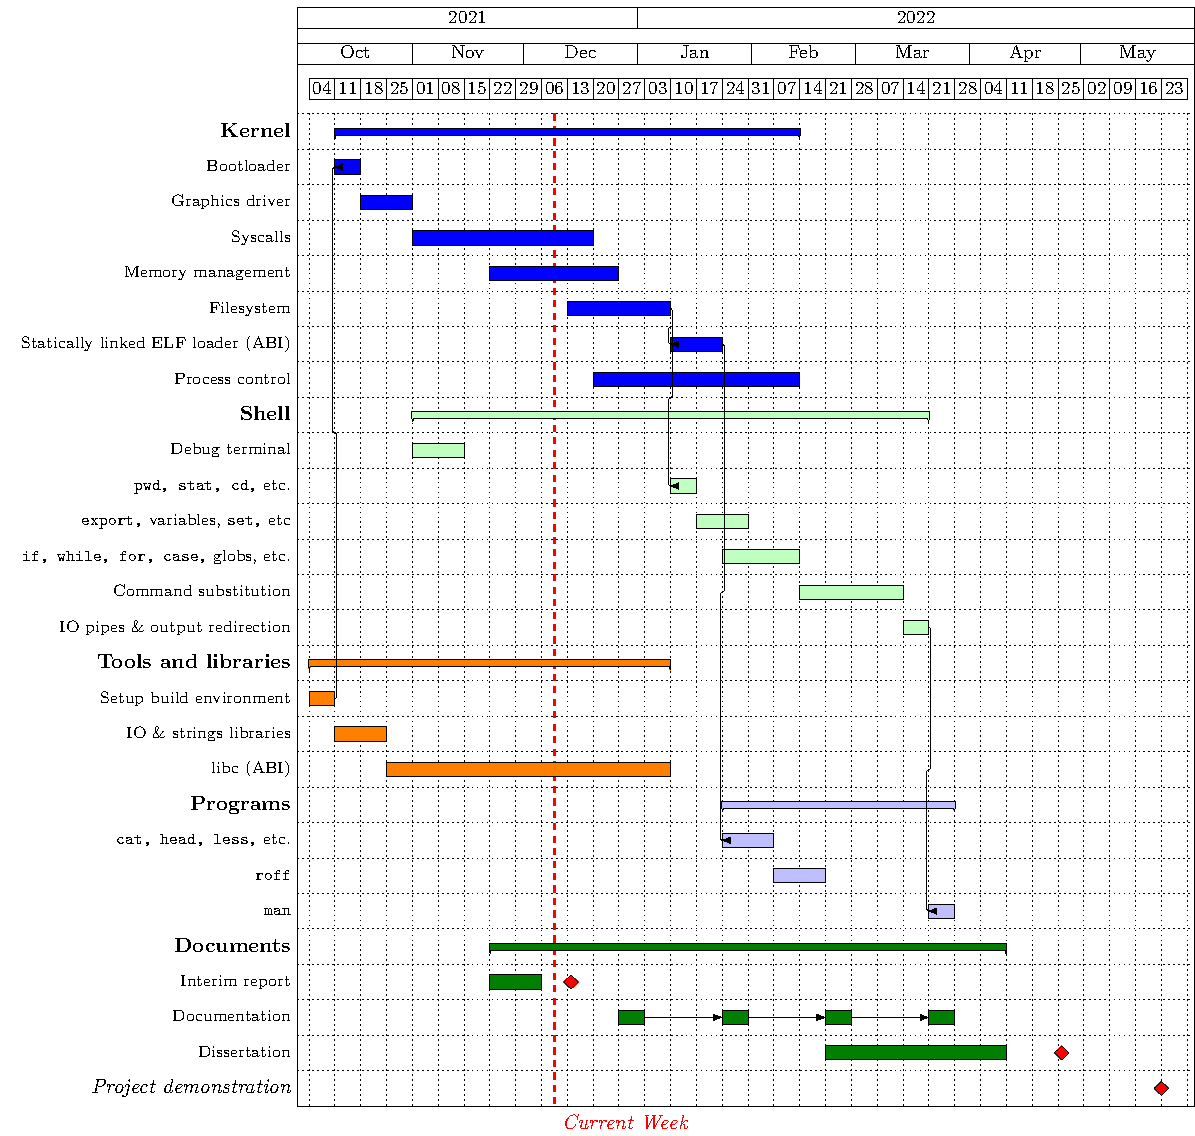
\includegraphics[scale=0.9]{build/interim-gantt.pdf}
    \caption{Gantt chart from the interim report}
    \label{fig:interim-gantt-chart}
\end{figure}


\clearpage
\section{Interim: Methodology}

\subsection{Software Development methodology}
The methodology I am using for the development of this project borrows
attributes from both \nameref{sec:cowboy_programming} and
\nameref{sec:agile_sw_dev}.

\subsubsection{Cowboy programming}
\label{sec:cowboy_programming}
Cowboy programming is a methodology categorised by being very free-form and not
having a very well-defined structure. It is often used by novice programmers
when they create solo projects, and it is the default when someone doesn't
think they are using any kind of methodology.

In cowboy programming, the developer has a lot of control over the project,
and they can decide the order features are implemented in, and even add or
remove features at will. The lack of planning causes development to follow the
developer's natural preferences, often leading to unfinished projects as the
developer gets to a stage where the only features left to implement are ones
the developer doesn't want to work on.

Cowboy programming is very well-suited to a solo development project, but it
comes with a lot of downsides and pitfalls. The best way to avoid these
development traps is to not completely rely on this methodology, but to also
integrate some aspects of Agile development.

\subsubsection{Agile software development}
\label{sec:agile_sw_dev}
Agile software development is a group of methodologies which all focus on
several core ideas. These are: frequent reviews of the product, lots of
planning and re-planning, a focus on good communication, and a very
well-structured development process. Some of the more popular Agile
methodologies include KanBan, SCRUM, Test Driven Development, and Extreme
Programming.

Agile development works best in situations with small development teams, and
some Agile methodologies involve pair programming, which requires two
programmers to work on the same code at the same time. I cannot use pair
programming or host team meetings, this being an individual project, but I can
still take inspiration from the techniques employed by different Agile
methodologies.

I will take inspiration from \gls{xp}~\cite{extreme-programming} and
\gls{tdd}~\cite{test-driven-development}. I will work from a list
of features which are organised by priority, which is an Extreme Programming
method. From \gls{tdd}, I will be writing developer tests and following
\gls{tdd} methods once the \gls{os} is mature enough to run tests in the
kernel.

\subsubsection{How I have been approaching the development until now}
The way that I have been developing the \gls{os} so far has been closer to
cowboy programming than to any agile software development methodologies. So
far, I have not started writing any developer unit tests for \gls{tdd}, as the
kernel has only just reached a stage where I could run tests on the emulator.

I have been loosely following the plan laid out in the Gantt chart from the
project proposal (\autoref{fig:original-gantt-chart} in the Appendix), but I
have not been using any other elements of \gls{xp}. The order in which to
develop the tasks has changed as I have been developing them, so I have been
exercising the freedom and control over the project that comes with cowboy
programming.

\subsubsection{How I intend to develop moving forwards}
Moving forwards in the development of the \gls{os}, I want to more closely
follow the intentions of agile development. I will try to use \gls{tdd}
wherever I can, writing developer tests at the start of each task in order to
have a clearly defined set of behaviour requirements for every feature.

\subsection{Software tools used to aid development}
\subsubsection{Source code editing}
For editing the source code of the \gls{os}, I am using the text editor
Vim~\cite{vim} with several plugins to assist me in writing correct code. I am
using the CoC extension~\cite{vim-coc} for autocompletion, and the clangd
language server~\cite{clangd} extension for CoC in order to provide source code
linting for C source files.

For source code formatting, I run the program
\texttt{clang-format}~\cite{clang-format} on the C source and header files. I
have defined a style guide for the project in a \texttt{.clang-format}
configuration file, which tells \texttt{clang-format} how to format my code.
This results in a consistent style throughout the entire project, causing the
source code to be easier to read and understand.

\subsubsection{\texorpdfstring{\glsxtrlong{rpi}}{RPi} 3 Emulator}
QEMU~\cite{qemu} is an emulator with out-of-the-box support for emulating the
host architecture. This means that on an \texttt{x86} machine, we can
emulate another \texttt{x86} machine. This isn't enough for emulating a
\gls{rpi}, as the \gls{rpi} uses the Aarch64 architecture. Thankfully, there is
a package on most linux distributions, ususally called something like
\texttt{qemu-arch-extra}, which adds support for other architectures. This
provides the program \texttt{qemu-system-aarch64}, which spins up an emulator
for Aarch64-based machines. The \gls{rpi} 3 is supported as a machine preset,
using the command line argument \texttt{-machine raspi3}.

The emulator can emulate everything about the \gls{rpi} except for the first
stage bootloader, which is the code that runs at the very start of the boot
process on a real \gls{rpi} and then loads the kerrnel (\texttt{kernel8.img}
for 64 bit mode). This bootloader is proprietary and runs on the \gls{rpi}'s
VideoCore GPU. I am not trying to develop a first stage bootloader, though, so
I do not need to worry about the lack of this functionality. The compiled
kernel is passed as an argument to the emulator when we start it
(\texttt{-kernel kernel8.img}). In the same way, we can give the SD card image
to the emulator, with the argument \texttt{-drive
file=sd.img,if=sd,format=raw}.

\subsubsection{Debugging}
GDB~\cite{gdb} is a debugger which can be used to debug executable programs.
Similar to QEMU only supporting one architecture by default, GDB only supports
running a program directly on the current machine. However, it does support
remote debugging with a commands once it has started (\texttt{target remote
URL:PORT}). Like with QEMU, there is an additional package which provides
support for additional architectures (\texttt{gdb-multiarch}). When we launch
QEMU, we can tell it to wait for a remote debugging session to connect before
it starts the emulator (using the commandline arguments \texttt{-s -S}). Once
QEMU is waiting for the debugger, we launch GDB (\texttt{gdb-multiarch
kernel8.elf} in a terminal) and then connect to the emulator as a remote
debugging client (using the GDB command \texttt{target remote localhost:1234}).

Now we can debug the \gls{os} kernel as if it is a regular program, using
breakpoints and disassembling it as we run through the execution. This is how I
debug the kernel when a new feature is not running as expected, and it allows
me to determine the cause of any issues more easily than a debug shell would
have done. Also, the debugger works without needing a working kernel, so I can
debug issues which cause the kernel to fail.

\subsubsection{Organising the build process}
When I first started this project, I was using CMake to automate the build
process. CMake is a tool which tries to automatically find the correct
dependencies required for compiling a project (the compiler, linker, and also
any libraries and included files can all be handled by CMake). Unfortunately,
CMake was causing issues with compiler and linker paths, and it was not
consistently finding the correct linker for the compilation of this project.

I then rewrote the build system using GNU Make (with a Makefile). This allowed
me to hardcode the correct compiler and linker for the build process, and I
haven't encountered any more issues with the compilation toolchain.

The top-level Makefile does not contain any rules to invoke the compiler
directly, and only handles the linking together of the compiled object files
into the final kernel. A separate Makefile is used to compile each source file,
and Make invokes itself recursively in each source directory for the
compilation.

The source files are kept separate from the object files and compiled kernel,
by putting all the results of compilation into a \texttt{build/} directory at
the top of the project (source files are located in \texttt{src/}). The object
files and final compiled binaries are also separated, with object files being
in \texttt{build/obj/} and binaries in \texttt{build/bin/}. Keeping the
directory structure organised in this way helps maintain an understanding of
the overall project structure as the project grows in size, as not keeping the
order in this way would result in quickly becoming overwhelmed by the sheer
number of files.

\section{Interim: Design}
\subsection{\texorpdfstring{\gls{os}}{OS} components}
\subsubsection{Features I expect to complete}
\begin{itemize}
    \item Microkernel with UART serial output and graphics driver for the \gls{rpi}'s
        HDMI video output. User interaction will use the display and read from
        the keyboard.
    \item Shell (hopefully POSIX-compliant) with scripting capabilities.
        Depending on time constraints, this may be a port of
        Dash~\cite{dash-shell}.
    \item Multi-process system allowing multiple processes to time-share the
        CPU with a process scheduler.
    \item An implementation of the System V ABI for executable files
        (statically compiled ELF files).
    \item Suite of core utilities (like those provided by GNU) - these may be
        partially or totally ported from the GNU
        coreutils~\cite{gnu-coreutils}.
    \item An init program for starting the \gls{os}'s essentials and for starting the
        root\footnote{Here, ``root'' means PID 0, not a root user (although if
        users are implemented, it would be both).} shell.
\end{itemize}

\subsubsection{Nice-to-haves}
\begin{itemize}
    \item A service manager for starting services at boot and ensuring that
        they remain running, restarting them if they fail. This may be bundled
        with the init system, like with systemd on most Linux distributions, or
        may be a separate program.
    \item Runs on hardware (not just a VM/emulator).
\end{itemize}

\subsubsection{Future possibilities}
\begin{itemize}
    \item A multi-user system with basic passwords and access control on files
        (file/directory ownership).
    \item A threads system with multithreading support (multiple threads owned
        by one process).
\end{itemize}

\subsubsection{\texorpdfstring{\gls{os}}{OS} components block diagram}
\autoref{fig:os-block-diagram} is a diagram of how the different components of
the \gls{os} will fit together. It shows how user programs running on the
\gls{os} would be supported by the \gls{os} components. The components
mentioned include user libraries (which would be included at
\texttt{/usr/include/} in the \gls{fs}), as well as various parts of the
kernel, such as system calls (see \autoref{sec:impl_syscalls}), the \gls{fs}
(\autoref{sec:impl_fs}), and the ``process control subsystem''. The ``process
control subsystem'' does not currently have any implementation, but it will be
made up of the parts of the kernel which control the processes that run on the
\gls{cpu} at any particular time.

\begin{figure}[htbp]
    \centering
    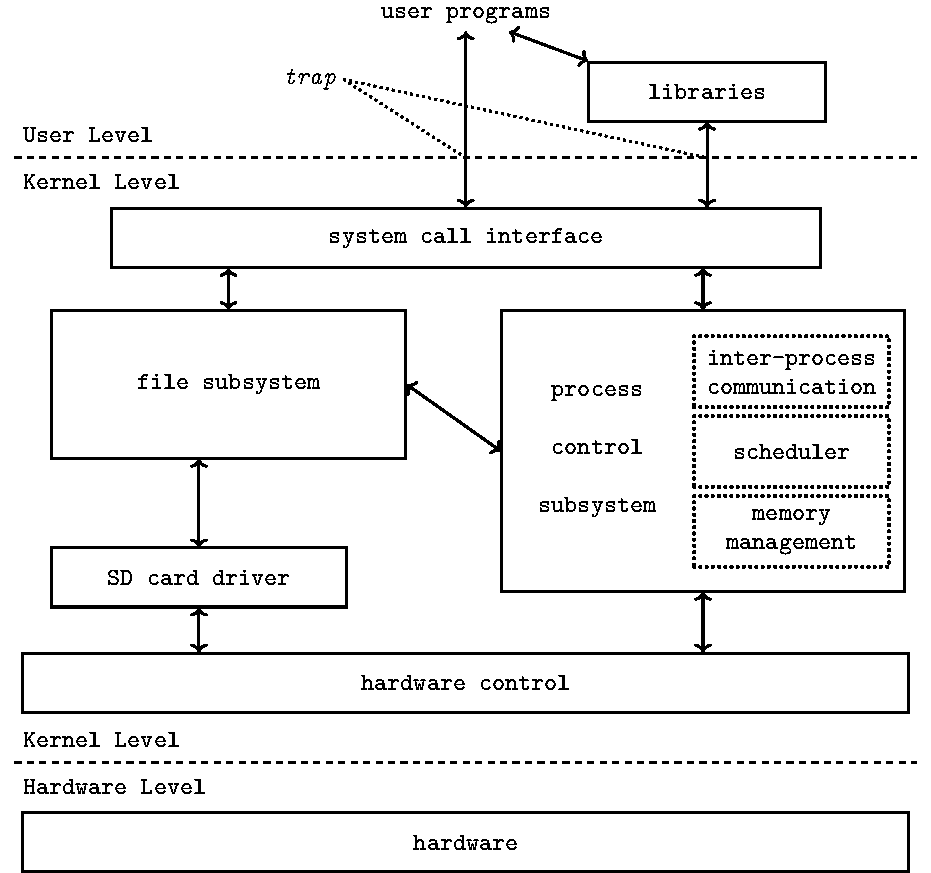
\includegraphics[width=0.8\textwidth]{build/os-block-diagram.pdf}
    \caption{A diagram of how the components of the operating system will
        interact with each other. Inspired by a diagram from a book on Unix
        (Figure~2.1 from~\cite{design-of-unix-os}). The versions of this
        diagram which are available online are low-resolution, so the version
        provided here is in a vector format, and this document's source code is
        available online~\cite{this-document}.}
    \label{fig:os-block-diagram}
\end{figure}

\subsection{Design of the shell and user interface}
\subsubsection{Shell}
The shell which I will include in the \gls{os} will be a port of a POSIX
compliant, simple shell, such as Dash~\cite{dash-shell}. This shell will be the
main way that users interact with the system, as it will allow them to execute
programs which do anything they need, such as compiling other programs, editing
text files, or viewing the contents of files. The shell will run in user space,
and any time it needs to run kernel-level functions, it will do so through the
system call interface. This is the same way the Bourne Shell ran on Unix, and
it is a known good way of allowing the user to control a computer. Anyone who
has experience with a shell will immediately feel at home when they see the
input prompt and a flashing cursor.

\subsubsection{User Interface and the graphics of the
\texorpdfstring{\gls{os}}{OS}}
The interface of the \gls{os} is the console. It is the text that is displayed
to the user from the \gls{rpi}. I will implement some quality of life features,
such as terminal scrollback, which allows the user to scroll up and see what
was printed to the terminal earlier. This feature reduces the need for a
terminal output pager such as \texttt{less}, which will not be implemented
until very late in the development.

The font I decided to use for the console is Bizcat~\cite{bizcat-font}. It is
an 8x16 bitmap font, and I converted it into a C source file as a constant
array. The font is easy to read at a screen resolution of 640x480, which gives
80 columns and 30 rows of text.

The colorscheme of the console is something that will likely change many times
during development, until I find something that I am completely happy with. At
the moment, the background is completely black, and the text is completely
white, but this would probably put strain on the users' eyes after using the
\gls{os} for a long time. I will experiment with color schemes once I have
implemented a program that can output a text file to the screen.

\section{Interim: Implementation}
\subsection{Programming languages used}
From the beginning of this project, I had already decided to write the majority
of the code for the \gls{os} in C~\cite{c-programming-language}. C is primarily
a systems implementation language (making it perfect for writing an \gls{os}),
and I was already very familiar with it, having used it regularly for the past
5 years.

For some very low-level parts of the \gls{os}, I needed to specify the exact
order in which I wanted \gls{arm} instructions to be executed, so ARMv8
assembly was the natural choice, being the closest language to the machine code
that gets executed without actually being the machine code. Assembly language
allows preprocessor macros, so I did not have to manually align instructions to
4-byte boundaries anytime there was a change, and header file ``include''s
which allow register values to be abstracted away from the logic and replaced
with meaningful names. These features were used extensively in the bootloader
and in \autoref{sec:impl_cpu_setup} for explaining the values placed into
various \gls{cpu} registers.

\subsection{Problems ecountered with the original implementation details}
At the start of development, I was using the GNU cross-compiler for bare-metal
\gls{arm} 64-bit targets, \texttt{gcc-aarch64-none-elf}. This was working but
the build system I was using at the time (CMake) was easier to configure using
clang/llvm as a cross-compiler. Also, the GNU cross-compilers are not available
in most Linux distributions' core repositories, so clang/llvm is much easier to
install, needing only the package manager of a Linux system.

Later in development, I was having difficulties maintaining the build system
which I had started the project with (CMake), as the intended usage is to
automatically detect the executables that should be used for compilation (the
cross-compiler, linker, etc.). This caused problems because if I modified the
status of my build computer, by installing some new packages for example, CMake
would detect and start using the wrong linker, causing the build process to
fail\footnote{I later discovered the cause of this. I had re-installed the
\texttt{gcc-aarch64-none-elf} cross-compiler, which resulted in the GNU
\gls{arm} 64-bit linker appearing before llvm's \texttt{ld.ldd}. CMake then
tried to use \texttt{gcc} (\textbf{not} the cross-compiler) to invoke the
linker, but the arguments for invoking the linker via \texttt{gcc} and
\texttt{clang} are different, so \texttt{gcc} was giving back an error, saying
that the \texttt{-T} argument was missing a parameter, and I was unable to
force CMake to call \texttt{ld.ldd} directly.}.

As a result of the problems I was having with CMake, I decided to use GNU Make
(with a \texttt{Makefile} instead of a \texttt{CMakeLists.txt}, calling the
\texttt{make} executable) instead. I created a Makefile for the project, and
this allowed me to hardcode the name of the compiler executable, and all the
tools needed to generate the compiled kernel image and SD card image. During
the implementation, as the number of source code files grew, I decided to start
using sub-make~\cite{sub-make} for compilation so that the main Makefile could
be kept simpler, so I moved the compilation commands into a separate Makefile
which handles each subdirectory of the main \texttt{src/} directory.

\subsection{Graphics driver}
\label{sec:impl_graphics}
For graphics, I created a simple library for manipulation of the framebuffer.
In order to print characters to the screen, I converted an 8x16 bitmap
font~\cite{bizcat-font} into a constant array definition in a C source file. I
then wrote a function to print a character from this array onto the
framebuffer, and I added global variables which keep track of the current
character position on the screen.

When the console reaches the end of a line, it moves to the start of the next
one. At the moment, when it reaches the end of the last line, it moves back to
the start of the first line. In the future I will implement scrolling, so that
when the console reaches the bottom of the screen, every line will be moved up
to make space for the next line.

\subsection{\texorpdfstring{\gls{cpu}}{CPU} setup}
\label{sec:impl_cpu_setup}
When the kernel starts, the \gls{cpu} will either be in \gls{arm-el} 2 or
\gls{arm-el} 3 (The \gls{rpi} only supports \gls{arm-el} 2 but I have written
code to support \gls{arm-el} 3 just for completeness). The boot code of the
kernel checks the current \gls{arm-el} and runs some code to put the \gls{cpu}
into \gls{arm-el} 1. The code sets up the system registers correctly to fake
the \gls{cpu} returning from an exception. When the registers are correctly
set, the \gls{arm} instruction \texttt{eret} is run, and the \gls{cpu}
``returns'' from the ``exception handler'', jumping into the kernel code and
entering into \gls{arm-el} 1. This is done in this way because exceptions are
the only way to change \gls{arm-el}, and the only way to reduce the
\gls{arm-el} is to perform an exception return (\texttt{eret}).

\subsection{System Calls}
\label{sec:impl_syscalls}
The system call interface requires writing an exception vector table. I created
an exception handler for the software interrupt instruction I will use to
trigger a system call (\texttt{svc \#0} in Aarch64 ARMv8 assembly). This is
incomplete at the moment, as I haven't yet worked out how I will locate the
correct function for a given system call.

I also wrote a basic exception vector table, but I was working from outdated
documentation, so I will need to update the table to have the correct padding
between the different exception types. I will also need to update the linker
script to place the exception vector table at the correct address in the
executable, or add code in the boot process to manually set addresses if
linking doesn't correctly set the addresses (the table is in low address space,
so it is possible that the bootloader will ignore anything so low in the kernel
executable).

\subsection{\texorpdfstring{\gls{fs}}{Filesystem}}
\label{sec:impl_fs}
I haven't made much progress on the \gls{fs} so far, as I was busy learning
what I needed to know about \glspl{arm-el} when I planned to implement the
\gls{fs}. Also, when I started working on the \gls{fs}, I discovered I had
overlooked the fact that I would need an SD card driver to be able to access
storage from the \gls{rpi}.

I took an existing driver for interfacing with an SD card (via the \gls{rpi}'s
eMMC controller) and integrated it into the kernel. I also copied some \gls{fs}
code from the same related work~\cite{rpi-boot-gh}, but I haven't finished
integrating anything related to a \gls{fs} into the \gls{os}. The virtual
\gls{fs} is unfinished, and so is the FAT \gls{fs}. This is one of the next
components that I will focus my efforts on.


\section{Interim: Progress}
\subsection{Project management -- Re-planning the project}
The original plan for the project was a little over-ambitious, which I
discovered as I was developing the current implementation. I have modified the
plan to account for the more restrictive time constraints, and also considering
my experience developing the \gls{os} so far. Some of the later, more complex
tasks have been removed from the plan, as I no longer believe I would be able
to complete them, and some tasks have been given more time.
\autoref{tab:interim-work-plan} shows the new plan for the project's tasks, and
\autoref{fig:interim-gantt-chart} is the Gantt chart which describes the dates on which
I expect to start and finish each of the tasks.

\subsection{Unexpected difficulties in development}
I have encountered several issues during development which I did not account
for in the original project plan. The first is not so much an issue as it is a
task not being required in the way that I expected. The \textbf{debug shell}
was not needed in the way I had planned to implement it. My plan was to prompt
the user for a command, and for the shell to support a very limited range of
commands, perhaps starting with a command to print the contents of a memory
address. This type of debugging has not been needed so far during the
development process, and I don't believe it will be needed, as I can use
\gls{gdb} for debugging memory locations, and \gls{gdb} doesn't even require
the \gls{os} kernel to be in a working state, which would be the most likely
scenario for if I would need to read memory.

The ``debug'' part of the debug shell task was still completed, as the current
version of the kernel prints debugging information to the serial port (and also
to the \gls{rpi} video output once the framebuffer is allocated). This
debugging information is changing as I add more features to the \gls{os}, and
lines which tested code that will not change again (i.e. the \texttt{printf}
function) are removed.

\textbf{System calls} were far more difficult to implement than I expected. The
way that system calls will be implemented is using \gls{arm} exceptions
to execute a function with the processor in a privileged mode of operation.
Unfortunately, when I started working on the system call implementation, I did
not have a very good understanding of the \gls{cpu} mechanisms by which
\gls{arm} processors handle exceptions. The \gls{cpu} will use a large number
of system registers, along with the current \gls{arm-el}, to decide where the
exception handler can be found, and in which \gls{arm-el} the \gls{cpu} should
handle the exception. I did not know any of this at the time that I started to
implement the system call mechanism, and I was using documentation for a very
old version of the \gls{arm} architecture. I did not even know which
\gls{arm-el} the \gls{cpu} was executing the kernel in, so I worked on code for
the \textbf{filesystem} for a while.

When I returned to working on system calls, I knew I needed to initialise the
\gls{cpu} state, so I followed a tutorial~\cite{raspberry-pi-os-gh} and used
the \gls{arm} developer documentation~\cite{arm-developer-regs} to learn enough
about \gls{arm} \glspl{arm-el} and exceptions. I wrote code to initialise the
\gls{cpu} into \gls{arm-el} 1, which I am going to use for the kernel of my
\gls{os}. I also set up the processor registers to correctly handle exceptions,
so that any system calls from either user space (\gls{arm-el} 0) or kernel
space (\gls{arm-el} 1) will both be handled by the kernel in \gls{arm-el} 1.

When I started working on the \textbf{filesystem}, I immediately realised
something that I forgot to consider for the original project plan. The
filesystem would require an SD card driver in order to interact with the
\gls{rpi} storage. I used an existing implementation of a simple \gls{rpi} SD
card driver~\cite{rpi-boot-gh}, which only required a small amount of
modification to get working. Once I had it integrated into my kernel, I created
an SD card image and added it to the emulator, then tested the driver to see if
it recognised the SD card. To my surprise, the driver knew when the SD card
image was present, and the initialisation function returned the expected value
when the image was present on the emulated \gls{rpi}.

My initial expectation of the difficulty of memory allocation was very
inaccurate. It is a much more complicated process than I had assumed it was,
and managing the memory that is allocated requires more kernel infrastructure
than I expected. As a result of this, memory management was brought forwards in
the list of tasks. However, I will need to finish implementing system calls
without a \texttt{malloc()} function. Programming without \texttt{malloc()} is
difficult and confusing, as functions must take pointers to data structures as
arguments. Results must be placed on the stack, as there is no heap. The
easiest way to implement \texttt{malloc()} is to use a system call
\texttt{mmap}, but my \gls{os} does not yet have a system call interface, so if
it turns out I need memory on the heap, I cannot implement \texttt{malloc()}
that way.

\subsection{Contributions and reflections}
The project's external sponsor (who is also my project supervisor), introduced
me to several of the related works~\cite{netBSD-git, riscOS-source}. He also
gave recommendations for some of the areas I was originally unsure of or less
knowledgeable about. He suggested that I implement the FAT \gls{fs} as it is
simple and relatively easy to implement, and he reminded me that on \gls{arm}
based systems, system calls would utilise software interrupts.

I think that the original project plan was too ambitious. I failed to consider
that I would have other modules and also extra-curricular obligations, and I
underestimated how much of my time would be taken up doing things unrelated to
the project. Overall, the project has not progressed as quickly as I had
originally expected. This is why I have scaled back the plan for the second
half of the year, replacing the shell and libc with ports of already existing
versions.

Now that I have reached a stage where I can more easily utilise techniques from
Agile software development (\autoref{sec:agile_sw_dev}), I will be able to more
successfully meet the deadlines I have set for the rest of the project. I
believe I have finished the most difficult part of developing the \gls{os}, as
I have learned a lot about \gls{arm} \glspl{cpu} and \gls{os} development best
practices. The rest of the project should be easier, as the most complex
systems are already implemented, but I will continue to put in as much effort
as I can, so that I can stay ahead of the new plan.


% End of main document - print glossaries, references, etc.
\printglossaries

% Mark each of our references as cited without actually citing them.
\nocite{osdev-wiki}
\nocite{unix-prog-env}
% Print the bibliography
\printbibliography[heading=bibintoc]

% FIXME: Appendices should NOT be a part of this file
\clearpage
\appendix
\pagenumbering{Roman}
\newrefcontext{appendix}
\newrefsection
\addcontentsline{toc}{section}{Appendices}
\renewcommand{\thesubsection}{\Alph{subsection}}
\renewcommand{\thesubsubsection}{\thesubsection.\alph{subsubsection}}

{\Large\bfseries Appendices\vspace{2ex}}

\subsection{Interim: Appendices}
\subsubsection{The original project plan}
This appendix contains all of the tables, figures, and diagrams from the
original project proposal, laying out my initial beliefs about what the project
entailed, and how much work each part of the project would take.

The diagrams are copied directly from the project proposal, so tenses may now
be incorrect (e.g. ``I think'' instead of the now more correct ``I thought''),
but this is done intentionally as this section is included only as a reference
to the content of the previous document.

\subsubsection{Work tasks}
Tasks are the individual components of the project, separated into the
components of the Kernel and Shell, the miscellaneous parts, and the documents
I will need to produce for the project. These tasks are enumerated in
\autoref{tab:original-work-plan} and then assembled into a Gantt chart in
\autoref{fig:original-gantt-chart}.

\begin{table}[H]
\begin{center}
\begin{tabular}{|l|r|}
    \hline
    Task & Duration (weeks)\\
    \hline \textbf{Kernel} &\\
    Bootloader & 1\\
    Graphics driver & 2\\
    Syscalls & 6\\
    Filesystem & 3\\
    Statically linked ELF Loader & 2\\
    Memory management & 4\\
    Process control & 8\\
    Init system and service manager & 5\\
    Threads and multithreading & 4\\
    \hline \textbf{Shell} &\\
    Debug shell & 2\\
    \texttt{pwd}, \texttt{cd}, \texttt{ls}, \texttt{stat}, etc. & 2\\
    \texttt{export}, variables, \texttt{set}, etc. & 2\\
    \texttt{if}, \texttt{while}, \texttt{for}, \texttt{case}, globs, etc. & 3\\
    Command substitution & 4\\
    IO pipes and output redirection & 1\\
    \hline \textbf{Misc parts} &\\
    Setup cross-compiler and build environment & 1\\
    IO and strings libraries & 2\\
    libc & 8\\
    \texttt{cat}, \texttt{head}, \texttt{less}, etc. & 2\\
    \texttt{roff} & 1\\
    \texttt{man} & 1\\
    \hline \textbf{Documents} &\\
    Interim report & 1\\
    Documentation & 5\\
    Dissertation & 7\\
    \hline
\end{tabular}
\caption{The original plan of work for the project, including how many weeks I
thought each component would take.}
\label{tab:original-work-plan}
\end{center}
\end{table}

\subsubsection{Gantt chart}
\begin{figure}[H]
    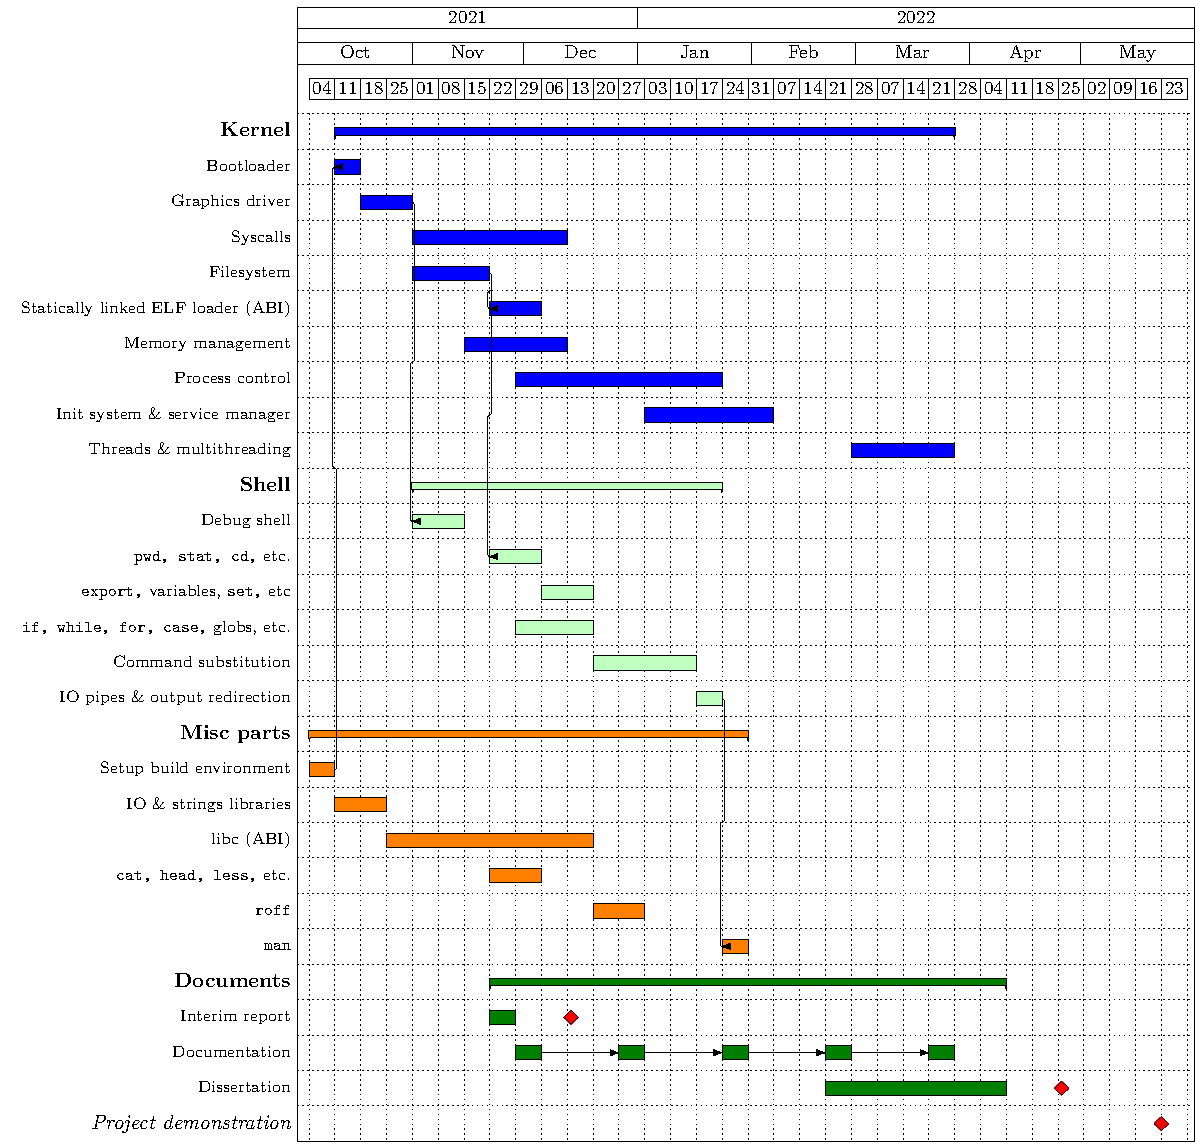
\includegraphics[scale=0.9]{build/original-gantt.pdf}
    \caption{A Gantt chart breaking down the proposed schedule of work for this
    project.}
    \label{fig:original-gantt-chart}
\end{figure}

\subsubsection{Work Packages}
A ``Work Package'' is a collection of tasks with a well-defined deliverable.
Not every task will be part of a work package, and some tasks will be work
packages on their own. \autoref{tab:original-work-packages} contains all of the
work packages for this project.

\begin{table}[H]
\begin{center}
\begin{tabular}{|p{45mm}|p{125mm}|}
    \hline
    \textbf{Work package} & \textbf{Description of the deliverable} \\
    \hline
    Debug shell using the graphics driver &
    A debug shell which is printed on the \gls{rpi}'s display and which uses
    keyboard input. The debug shell should accept several commands for
    debugging the processor status (including, but not limited to, printing the
    contents of memory, writing to memory, and jumping to a given memory
    address).
    \\ \hline
    A basic kernel which can load (from disk) and jump into a compiled \gls{elf}
    program. &
    A program that can load a statically compiled \gls{elf} executable binary
    into memory and then jump to its entry point. This requires a filesystem
    library to be implemented, and also includes the \gls{elf} loader task.
    \\ \hline
    Scheduling algorithm &
    A scheduling algorithm with support for multiple processes running on the
    system concurrently. This will include an implementation of
    \texttt{fork(3)} or a similar function in order to spawn new processes and
    \texttt{execve(2)} to replace the current program with a new process.
    \\ \hline
    Init system and service manager &
    An init system which is run at boot and starts all necessary parts of the
    \gls{os} and then spawns the root shell. The service manager ensures that
    all desired daemons and processes are started at the correct times and
    remain running, restarting them if they die.
    \\ \hline
    A shell &
    A (POSIX-compliant) shell \textbf{or} a port of a simple shell like
    Dash\cite{dash-shell}. If I decide that implementing my own POSIX-compliant
    shell is too large of a task, then I will port the source code for Dash to
    run on my \gls{os}, implementing the required syscalls to get it working.
    This shell will be the main way users interact with the \gls{os}.
    \\ \hline
    Documentation &
    This package contains several parts. I will create documentation for how
    each part of the \gls{os} works, and a guide for how new programmers can get
    started developing programs for the system. The documentation will be
    completed in stages as I develop the \gls{os}, and I will go back
    to keep it up-to-date as I make changes to components and add new
    components.
    \\ \hline
    Multithreading support and multi-core scheduling &
    The \gls{rpi} 3 has 4 \gls{cpu} cores. This work package will enable users
    to take advantage of the additional processing power of the other 3 cores
    for their programs. This includes a threading library similar to
    \texttt{pthread} on Linux systems, and improvements to the scheduler so
    that it can give different \gls{cpu} cores to multiple threads owned by the
    same process. \textbf{This work package is optional}.
    \\ \hline
\end{tabular}
\caption{The work packages of the project and their deliverables.}
\label{tab:original-work-packages}
\end{center}
\end{table}

\clearpage
\subsection{Gantt chart}

\begin{figure}[H]
    \centering
    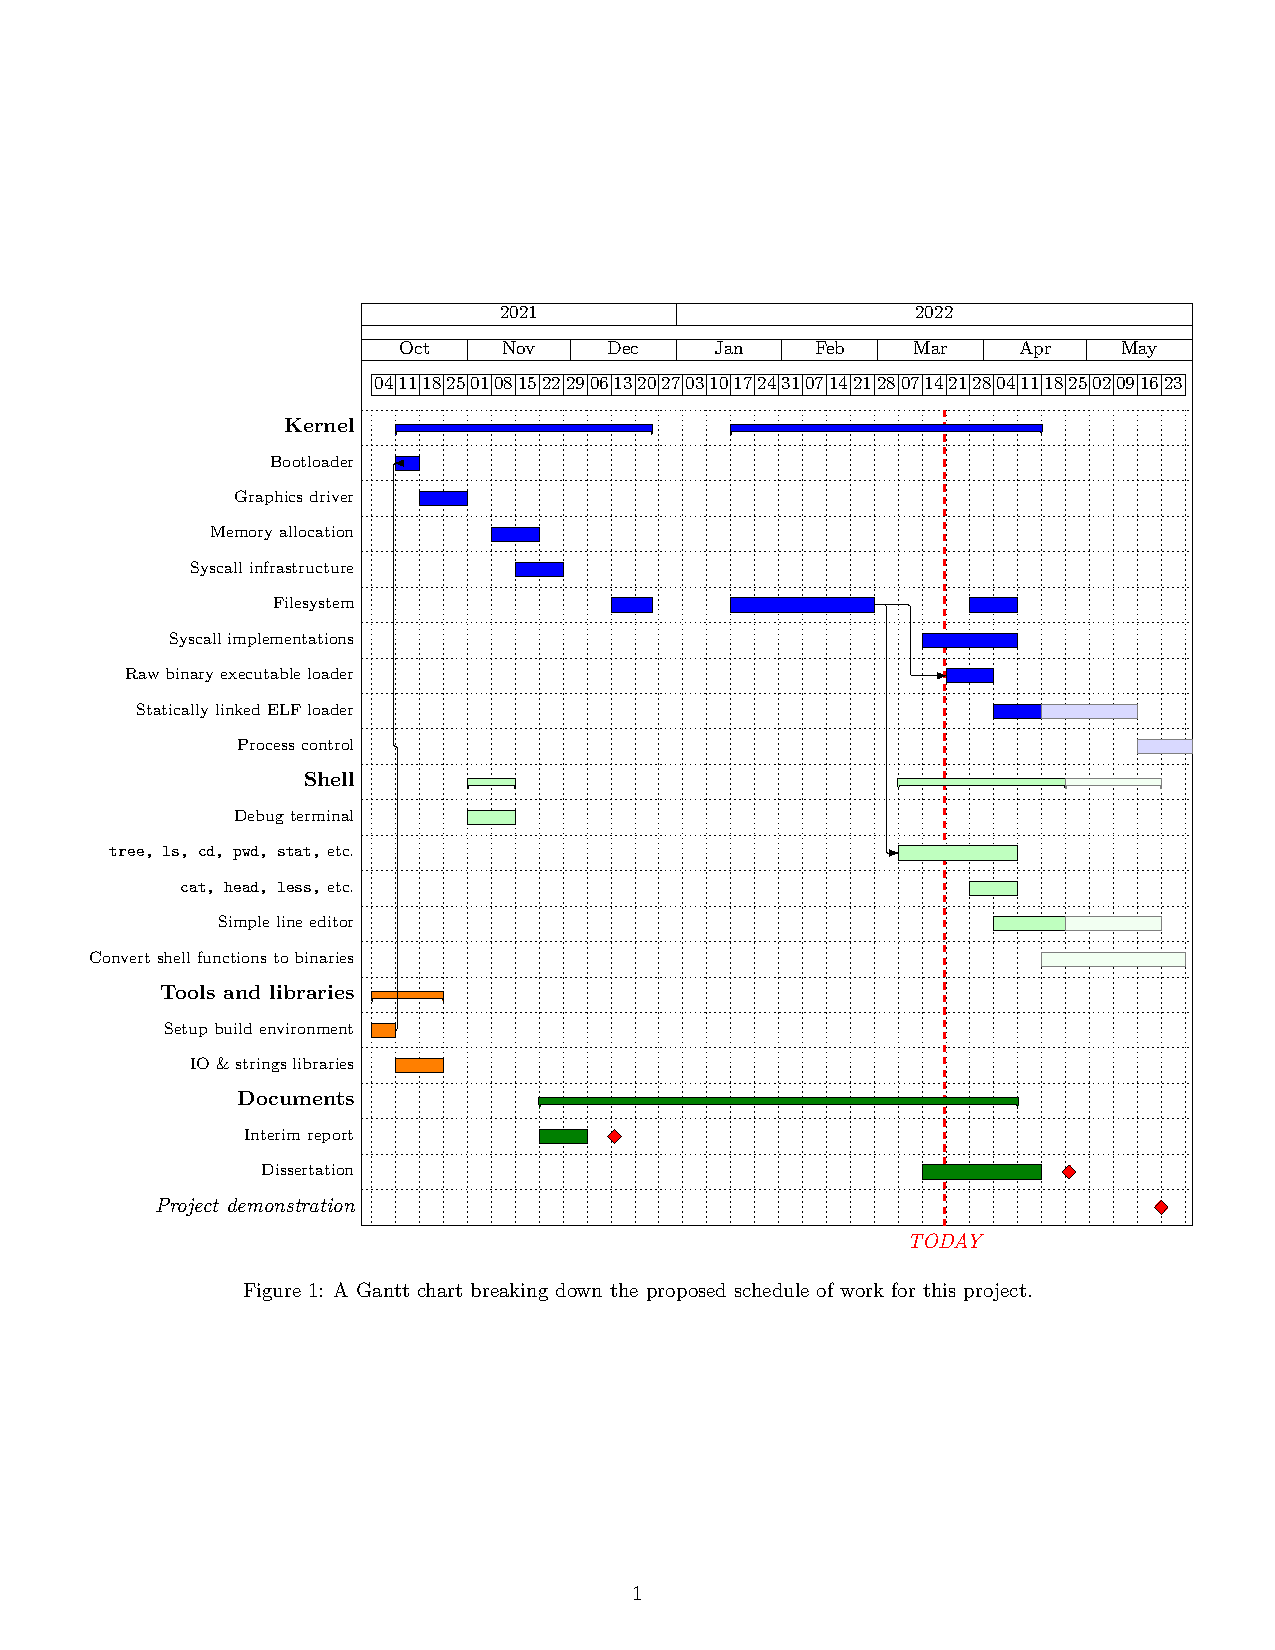
\includegraphics[scale=0.9]{build/gantt.pdf}
    \caption{A Gantt chart breaking down the proposed schedule of work for this
    project.}
    \label{fig:gantt-chart}
\end{figure}

\subsection{Future plans block diagrams}

\begin{figure}[H]
    \centering
    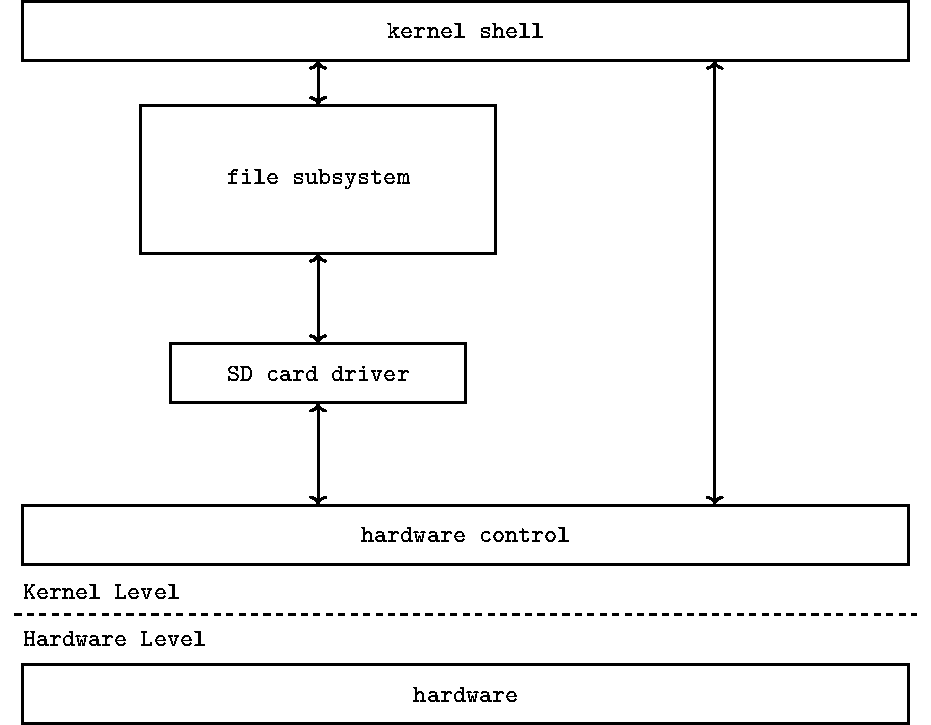
\includegraphics[width=0.32\textwidth]{build/finished-block-diagram.pdf}
    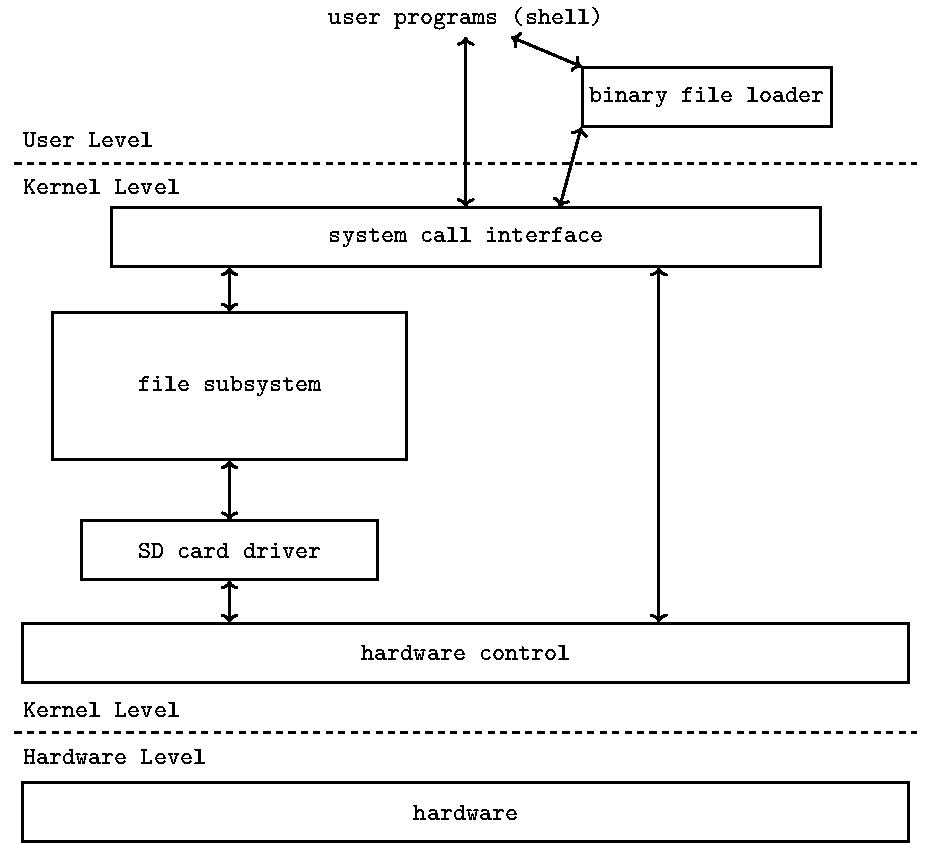
\includegraphics[width=0.32\textwidth]{build/nextstep-block-diagram.pdf}
    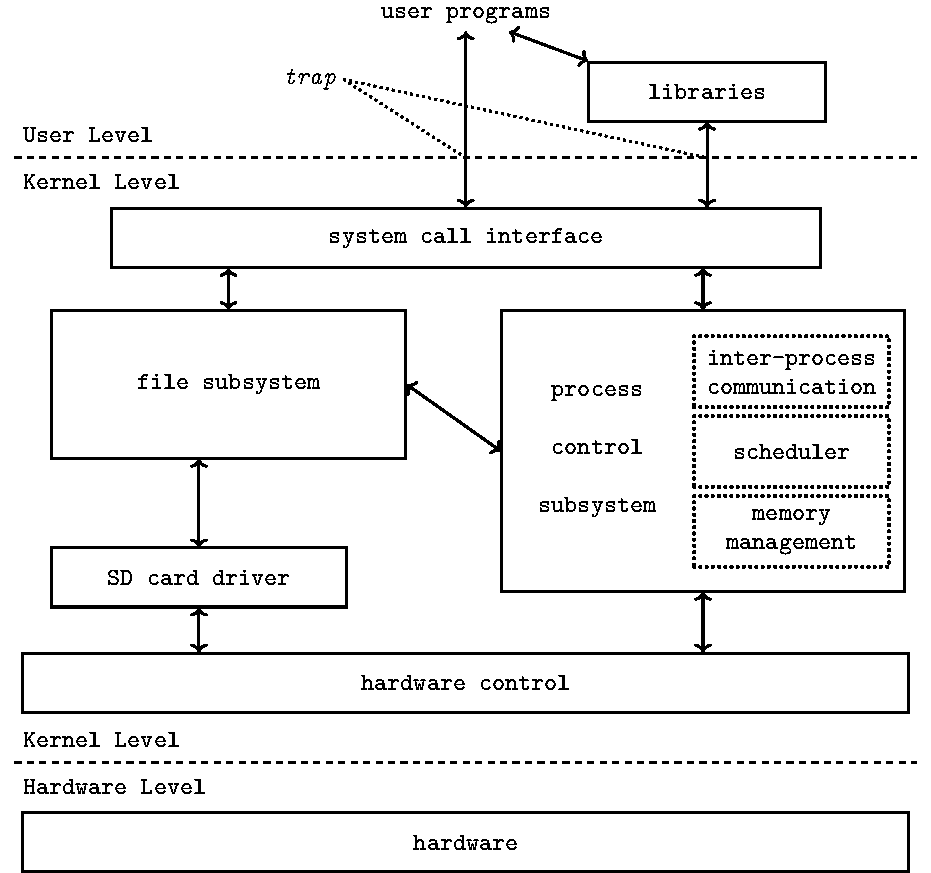
\includegraphics[width=0.32\textwidth]{build/os-block-diagram.pdf}
    \caption{My current estimation for how future development would work on
        this project. On the left is the current state of the Operating System.
        On the right is the diagram of how the Unix system was structured.}
\end{figure}

% End of main document - print glossaries, references, etc.
\printglossaries


\end{document}
